% 1977 年云南卷第 6 题：直角三角形 ABC 内接于外接圆，斜边 AB 为直径 2R，
% 直角在 C（带直角标记），锐角 β 在 B 处（按源卷第 3 页布局）
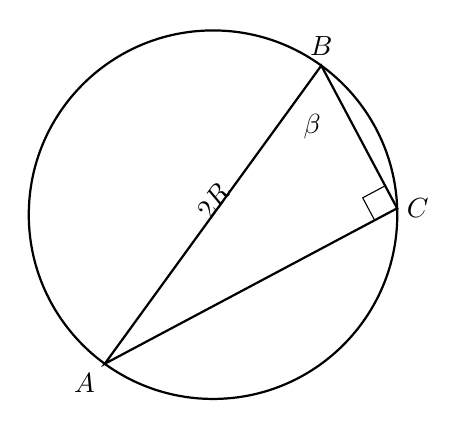
\begin{tikzpicture}[scale=1.8]
  \draw[thick] (0,0) circle (1.3);
  \draw[thick] (-0.764,-1.052)--(0.764,1.052)--(1.299,0.045)--cycle;
  \draw[thin] (1.140,-0.039)--(1.056,0.119)--(1.215,0.204);
  \node[below left] at (-0.764,-1.052) {$A$};
  \node[above] at (0.764,1.052) {$B$};
  \node[right] at (1.299,0.045) {$C$};
  \node[rotate=54] at (0,0.10) {$2R$};
  \node at (0.70,0.62) {$\beta$};
\end{tikzpicture}
